\documentclass{report}

\usepackage[utf8]{inputenc}
\usepackage[T1]{fontenc}
\usepackage[francais]{babel}
\usepackage{graphicx}
\usepackage{lmodern}
\usepackage{amsmath}
\usepackage{amssymb}
\usepackage{mathrsfs}
\usepackage{geometry}
\geometry{scale=0.8, nohead}

\author{Gautier \bsc{Dakin}, Nicolas \bsc{Ehrhardt}, Lucas \bsc{Plaetevoet}}
\title{Projet Gherkin}

\begin{document}
\maketitle

\section*{Introduction}
L'objectif du projet est de réaliser un lecteur audio intelligent. Il part d'un constat simple, nous possèdons tous trois une librairie audio conséquente ; et bien que nous ayons chacun notre préférence pour un lecteur audio, aucun d'entre eux ne nous satisfait pleinement.

Trois axes nous intéressent principalement :
\begin{itemize}
\item L'affichage : en effet, nous souhaiterions trouver le meilleur compromis entre interface minimaliste, et fonctions essentielles. Ceci en s'adaptant à l'environnement de bureau Ubuntu basé sur Unity. En cela, nous nous sommes d'abord basés sur l'interface du lecteur par défaut Rhythmbox qui nous paraissait un bon point de départ.

\item L'intelligence : plusieurs grandes sociétés ont travaillé sur la lecture intelligente et la proposition de chanson en lien avec les goûts de l'utilisateur. L'un des objectifs est de trouver des solutions pour proposer un mode de lecture intelligent et ne demandant aucun effort à l'utilisateur.

\item Les performances : le dernier grand axe est la recherche de performances ( c'est-à-dire pourcentage d'utilisation du processeur minimal ). Les performances du serveur audio MPD étant de ce point de vue tout à fait intéressantes, nous serions enclin à pousser le développement du projet suivant cette architecture.
\end{itemize}

\section*{L'interface}
\subsection*{Orientation du projet}
Comme sus-mentionné nous avons basé notre interface sur celle du lecteur audio par défauti (type Rhythmbox, de sorte à ne pas perturber les habitudes de l'utilisateur). Mais un constat s'impose : Aujourd'hui, les écran 16/10 voire 16/9 sont légions et majoritaires ; Ubuntu, à travers unity, à décidé de tirer parti de ce nouvel état de fait pour proposer un menu latéral. Les arguments sont : gain de place, minimalisme. Le principal problème étant que ce menu empiète parfois sur les boutons des applications en plein écran lorsque celui-ci se dévoile.

Pour répondre à cette problèmatique, nous proposons un menu à droite de notre application. Optimisant ainsi la place, et évitant cette gène.

\subsection*{Développement}
La librairie PyQt4 sur laquelle se base le lecteur nous a permis de développer rapidemment cette interface. Le développement de l'interface s'est fait en trois temps :
\begin{enumerate}
\item On crée dans un premier temps une première interface graphique grâce à QtDesigner. Cette application permet d'avoir une vision en WYSIWYG de l'interface, et donc d'éviter les erreurs de goûts et de mauvais placement.
\item On modifie légèrement le code généré par QtDesigner pour rajouter quelques fonctionnalités. (Ex : Gestion des îcones)
\item On sépare le fichier en deux .py. Un premier contient le code légèrement modifié obtenu via QtDesigner. Le second va gérer toutes les modifications de l'interface graphique, ainsi que la gestion des signaux et slots de Qt. (Ex : l'update de la barre de progression, lié le PlayButton à la fonction play() )
\end{enumerate}

\begin{figure}[h]
\centering
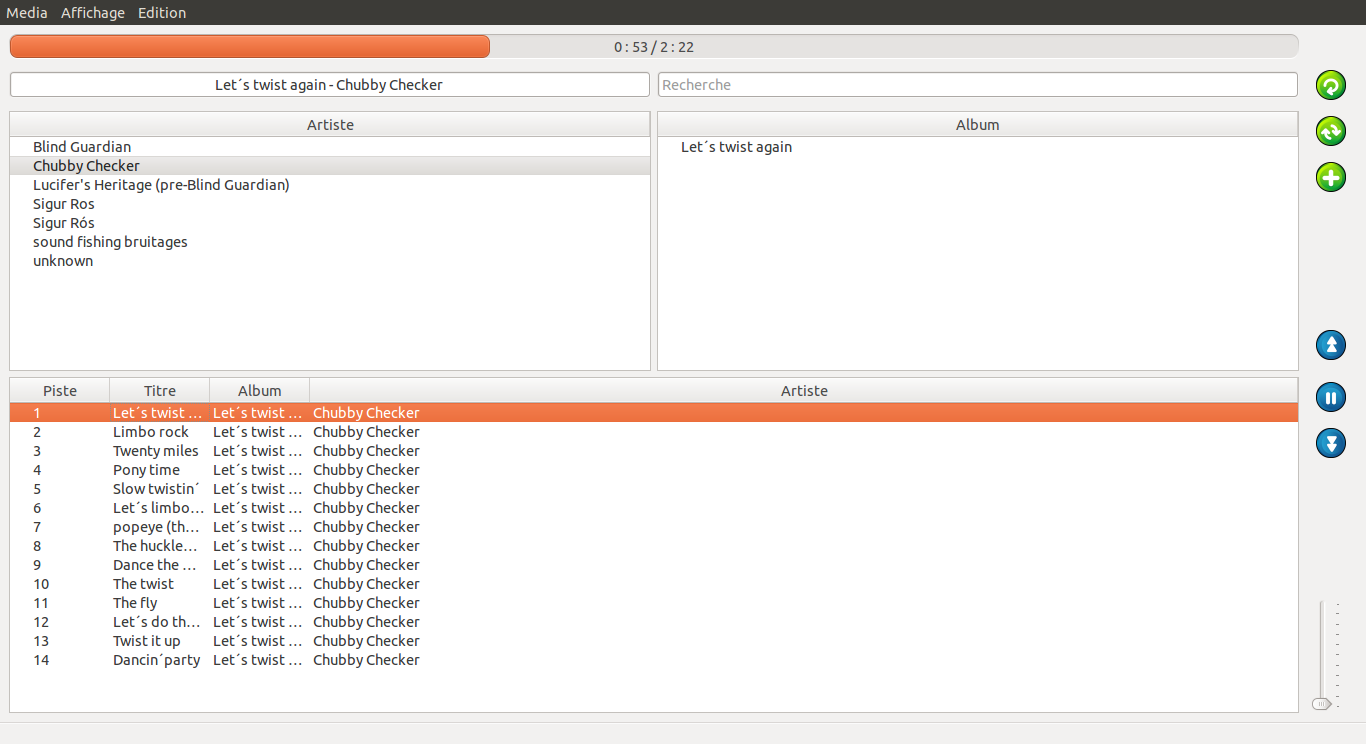
\includegraphics[scale=.3]{interface.png}
\caption{Interface graphique du lecteur.}
\end{figure}

Quelques interrogation demeurent cependant : quid des performances ? Pourrait-on segmenter plus encore le code ?

Nous ne sommes qu'au début de la pleine maitrise de cette librairie. Ainsi, si nous utilisons des "signaux" et des "QThread" il nous faudrait probablement revoir certaines fonctions peut être un peu trop gloutonnes ( néanmoins fonctionnelles ).

\section*{L'intelligence}
\subsection*{L'idée}

L'idée de l'intelligence est simple en elle-même. Elle a pour but de mettre des probabilités sur le passage entre deux chansons. Exemple : Vous êtes actuellement entrain d'écouter la "Sonate au Clair de Lune". Théoriquement, la probabilité d'avoir envie d'entendre/écouter "Highway to Hell" après la "Sonate au Clair de Lune" est extrêmement faible (sauf si cela est dans vos habitudes)
Si, au contraire, après la sonate de Beethoven, l'utilisateur a tendance à écouter le "Requiem" de Mozart, alors la probabilité de passage entre ces deux chansons sera d'autant plus grande.

Cette vision de passage d'une chanson à l'autre entre exactement dans le cadre théorique des chaînes de Markov où l'on a une matrice P tel que $P(x,y)$ représente la probabilité de passage de l'état x à l'état y.

\subsection*{Développement}

On a donc l'idée de représenter les transitions entre deux pistes audio par une chaine de Markov. Reste à savoir comment l'implémenter. Imaginons une bibliothèque moyenne sur un ordinateur. On tourne autour de 4000 ~ 5000 pistes audio. Gérer en permanence une telle matrice est extrêmement lourd, or on recherche en premier la rapidité d'exécution. On développe donc comme suit :

\begin{itemize}
\item
On crée un dictionnaire de nom markov, tel que markov[i][j] renvoie la probabilité de passage de i à j si elle existe.
\item
On pondère ces probabilités par un nombre dépendant uniquement de i. Ce choix implique qu'on considère qu'à un temps très élevé, on a théoriquement convergence vers la playlist idéale pour l'utilisateur. Cela ne signifie pas pour autant que la playlist devient déterministe. On a juste théoriquement élagué les probabilités très faibles pour ne laisser plus que les probabilités plus importantes. On a donc en théorie une convergence vers un arbre de probabilité plus ou
moins stable par utilisation de Gherkin.
\item
Selon certains critères, on décide d'incrémenter ou de décrémenter la probabilité, en gardant le caractère stochastique de markov. On incrémente ainsi la probabilité lorsque l'on réalise l'écoute entière d'un morceau, on incrémente la probabilité entre le morceau précédent et ce morceau. Lorsque l'utilisateur décide de passer une chanson, on abaisse la probabilité de passage entre le morceau précédent et le morceau qui vient d'être sauté. Enfin, on décide
d'incrémenter la probabilité lorsqu'un morceau est double cliqué, ce qui peut permettre à l'utilisateur de configurer en quelques instants ces playlists.
\item
Régulièrement, on enregistre le dictionnaire markov sur le disque dur. Enfin d'éviter de revenir au cas de la matrice, les probabilités trop faibles ($ < \epsilon$) sont élaguées c'est-à-dire qu'elles sont suppriméees et rajoutées équiprobablement sur les autres clefs du dictionnaire. Cet élagage permet de réduire le nombre de clefs du dictionnaire et donc de garantir une taille plus faible.
\end{itemize}



\section*{La gestion de la librairie}

Une petit librairie d'outillage à été créé pour l'occasion. Elle effectue trois taches basiques :
\begin{itemize}
\item la création d'un fichier XML recensant les fichier audio d'un dossier et leurs tags.
\item la mise à jour du fichier XML ( en développement ).
\item le chargement du fichier XML par l'interface graphique pour l'affichage et l'intelligence.
\item la création d'une playlist de lecture classique.
\end{itemize}

\section*{Le serveur}

\subsection*{Description}

Le serveur audio est complètement indépendant de l'interface graphique. Il ne prend en argument que le chemin d'une chanson. On peut ensuite :
\begin{itemize}
\item jouer;
\item mettre en pause,
\item arrêter,
\item obtenir le temps de lecture,
\item obtenir la longueur de la chanson jouée.
\end{itemize}

Celui-ci est basé sur la librairie média d'ubuntu par défaut : Gstreamer. Une fois de plus, il s'agit de se plonger dans la documentation de cette librairie, ce qui est un travail très fastidieux et parfois pénible.

\subsection*{Futur}

Le serveur est pour le moment plutot énergivore, il a besoin d'un certain nombre d'optimisation. En outre, l'on pourrait avoir envie de regrouper l'intelligence dans ce même serveur ( dans une sur-classe ? ) pour permettre le fonctionnement de l'application en mode console seulement et gagner en ressources.

\end{document}
